\documentclass{article}
\usepackage[utf8]{inputenc}
\usepackage{graphicx}
\usepackage[a4paper, portrait, margin=2.5cm]{geometry}
\usepackage{amsmath}
\usepackage{float}
\usepackage{wrapfig}
\usepackage{subcaption}
\usepackage{hyperref}
\usepackage{placeins}

\setlength\parindent{0pt}

\begin{document}

\begin{titlepage}
    \begin{center}
        \vspace*{1cm}
        \Huge
        \textbf{Optical Tweeweeweeweezer}
    
        
        \vspace{0.5cm}
        \LARGE
        Advanced Lab Course
        
        \vspace{1.5cm}
        \textbf{Louis-Hendrik Barboutie (020157041C), Frederik Ehl (0201719742) and Florence Schmerber (0201845640)}
        
        \vspace{1cm}
        Supervisor: Sergey Ershov
        \vfill
        

        
\includegraphics[width=0.4\textwidth]{logo_uni.jpg}
        
        \Large
        $28^{\underline{\text{th}}}$ March 2022
    \end{center}
\end{titlepage}


\section{Introduction}
Optical tweezers is a scientific instrument that uses a highly focused laser to trap and move around small particles. The optical tweezers experiment was a Nobel Price winning experiment by Arthur Ashkin in 2018, 48 after his paper called "Acceleration and Trapping of Particles by Radiation Pressure" was released.\\
This method is actively used in biology and medicine, for example to grab specific cells or bacteria.\\
We will carry out the same experiment with a focus on the study on the Brownian motion of the particles. Then, when using the laser to trap a particle, will be using the Mie regime, where the size of the particle is larger than the wavelength of the laser beam, in contrast to the Rayleigh regime, where the opposite is the case.

\section{Theory}

\subsection{Particle trapping with a laser}

\begin{wrapfigure}{r}{0.4\textwidth}
    \centering
    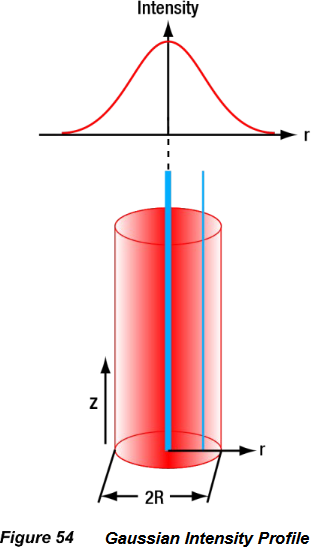
\includegraphics[width=0.2\textwidth]{gaussianLaser.png}
    \caption{Gaussian profile laser}
    \label{fig:gaussianLaser}
\end{wrapfigure}

The laser used in the experiment has a gaussian profile, ie. the intensity of the light is not constant alongside a cross section of the beam. It is highest at the center of the beam and then decays towards the edges. A schematic representation is depicted in fig.~\ref{fig:gaussianLaser}. Individual light beams composing the total light beam are parallel to each other. \medskip

In order to trap a particle with a laser, the laser has to hit the particle. When the laser comes in contact with a particle, several phenomena occur. The most important one, is the refraction of the beam. The laser beam will first travel in air, with optical index $n_{air}$, and then be refracted on the surface of the particle which has a refractive index $n_{particle}>n_{air}$. By Snell's law the beams will be bent towards the normal of the surface where the beam hits the particle. Since the particles are spheres, the beams will always be bent inwards. \medskip

When the light beam gets refracted, its direction changes, and therefore its velocity and momentum change. By momentum conservation, the change in momentum is transferred to the particle. This can be simply modeled with a vector model, comparing two individual light beams for an unfocused laser. Two cases must be differentiated though: when the light beams are symmetric to the center axis of the laser beam, and when they are not. The vector representation of the refraction is depicted in fig.~\ref{fig:unfocusedLaserMomChg}. The total change in momentum is then represented in fig.~\ref{fig:unfocusedLaserMomChg}.

\begin{figure}[!ht]
    \centering
    \begin{subfigure}{0.49\textwidth}
        \centering
        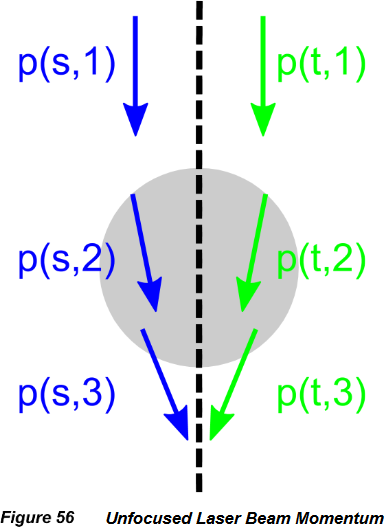
\includegraphics[height=0.5\textwidth]{laserSymmetricalBeams.png}
    \end{subfigure}
    \begin{subfigure}{0.49\textwidth}
        \centering
        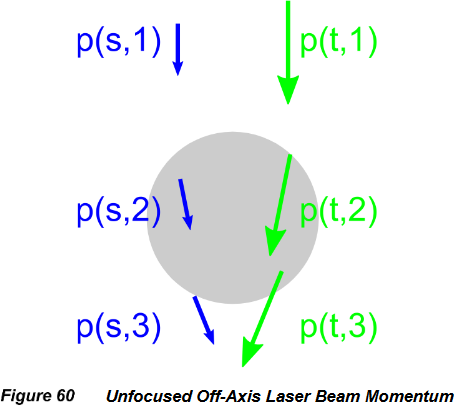
\includegraphics[height=0.5\textwidth]{laserAsymmetricalBeams.png}
    \end{subfigure}
    \caption{Vector representation of the momentum of individual light beams passing through the particle}
    \label{fig:unfocusedLaserMomChg}
\end{figure}
\FloatBarrier

\begin{figure}[!ht]
    \centering
    \begin{subfigure}{0.49\textwidth}
        \centering
        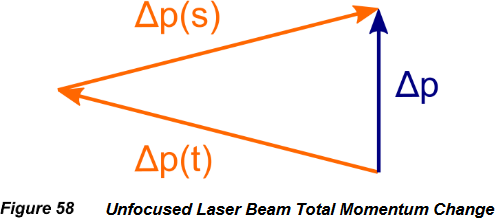
\includegraphics[height=0.5\textwidth]{momentumChangeSymmetricLaser.png}
    \end{subfigure}
    \begin{subfigure}{0.49\textwidth}
        \centering
        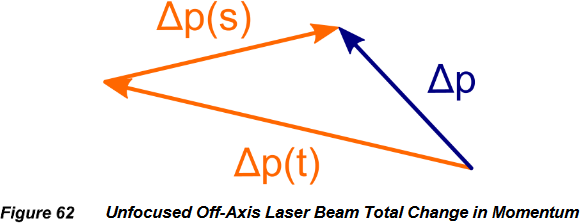
\includegraphics[height=0.5\textwidth]{momentumChangeAsymmetricLaser.png}
    \end{subfigure}
    \caption{Vector representation of the change in momentum of the individual light beams}
    \label{fig:unfocusedLaserTotMomChg}
\end{figure}
\FloatBarrier

By momentum conservation, the particle has a change in momentum going the opposite direction. In this case, the momentum points away from the central axis of the laser beam and points down. An unfocused laser beam therefore cannot trap a particle. Only a focused laser beam can work as a trap. 

\begin{figure}[!ht]
    \centering
    \begin{subfigure}{0.49\textwidth}
        \centering
        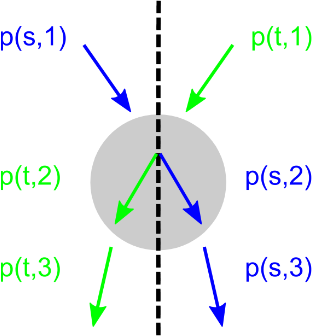
\includegraphics[height=0.5\textwidth]{laserFocusedBeam.png} 
    \end{subfigure}
    \begin{subfigure}{0.49\textwidth}
        \centering
        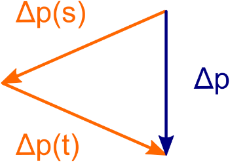
\includegraphics[height=0.5\textwidth]{momentumChangeFocusedBeam.png}
    \end{subfigure}
    \caption{Vector representation of the change in momentum of the individual light beams for a focused beams}
    \label{fig:focusedBeam}
\end{figure}
\FloatBarrier

As one can see in fig.~\ref{fig:focusedBeam}, the change in momentum for light focused inside the particle is toward the bottom, therefore the particle has a change in momentum upwards. In addition, for off-axis beams, the change in momentum is towards the center of the laser. This can be used as a "trap", so that the particle wants to stay inside the laser beam. While the representations are two dimensional, this also holds true in three dimensions due to the isotropic nature of the laser beam. An important note on this representation is that the momentum only changes direction and not value. When we compare the vertical component of the momentum before entering and after exiting the particle, we observe the following: in the unfocused case, the vertical component is greater before, so it pushes the particle down, while in the focused case it is greater after, and propulses the particle upwards. This generates the \textit{gradient force}. \medskip

Other phenomena occurring are absorption and reflection of the light. These have to be sufficiently small so that the trapping is still possible. Their sum is the \textit{scattering force}, acting in opposite direction to the gradient force. Gravity can also be neglected ($g=0$, à la Henkel), since the particles are suspended in a liquid solution. \medskip

The maximum holding force of the laser can be determined. It has to compensate the Brownian motion and the frictional force. In fact, in the liquid, only friction forces act on the particles. This force is only proportional to the speed of the particle and given by:
\begin{equation}
    F_{\text{friction}} = 6 \pi \eta_{eff} R v
    \label{eq:friction}
\end{equation}
Where $v$ is the speed of the particle and $R$ its radius. $\eta_{eff}$ is the viscosity of the solution. 

There is no formula for the true maximum holding force of the laser, but we can determine the maximum observed holding force, which is given by eq.~\ref{eq:friction} when $v=v_{max}$. This is when the friction force is highest, and if the laser still traps the particle, its holding force is greater than the friction force value (and opposite in direction).

\subsection{Brownian motion}
The Brownian motion is the random vibrating movement of free particles in a medium such as liquids or gases. Much stronger random displacements of a particle can be detected with smaller particle sizes, less viscous mediums and with higher temperatures. The Brownian motion is regarded as a diffusion process. For an isolated particle, with no action with neighbouring particles, its diffusion coefficient, D, can be expressed as the Stokes-Einstein equation:
\begin{equation}
    D = \frac{k_BT}{6\pi\eta R}
\end{equation}
With $k_B$ being the Boltzmann constant, T the temperature in Kelvin, $\eta$ the viscosity of the medium and R the radius of the particle.

\subsection{Rayleigh scattering regime and Mie regime}
In the Rayleigh regime the radius R of the particle is considerably smaller than the wavelength of the incident laser beam. The particle can be assumed to be dielectric and thus each particle has an induced dipole moment $\Vec{p}$. Since the radius is much smaller than the wavelength of the beam, the electrical field is approximately spatially constant, meaning that the induced dipole moment is equally strong for each particle. As a result, the polarization $\Vec{P}$ arises. The polarization is proportional to the electrical field, just as the potential energy U, as well as the intensity I, is proportional to $|\Vec{E}|^2$.\\
The gradient force, is therefore expressed as:
\[ F_{grad} = \frac{2\pi \alpha}{cn_m^2} \nabla I\] Where $\alpha$ is the polarizability of the dipoles, $n_m$ the refraction index of water and $\nabla I$ the intensity gradient.\vspace{0.5cm} 

The Mie regime on the other hand, uses not a dipole approach, but rather a geometrical optics approach. Since the radius of the particle is larger than the wavelength, conditions of geometric optics are fulfilled. We then assume that the the laser beam consists of a bundle of rays. Since, light, that is photons, can transfer momentum to an object, the force action of a beam is then simply the change in momentum of particle over time.
\[ F = \frac{dp}{dt} \]
As the beam hits the particle, part of the light will be reflected and part of it will be transmitted. The same happens inside the particle, when the light hits its internal wall. Once the beam exits the particle it will have undergone a change in velocity, and therefore also a change in its momentum. The force of the particle, as stated above, is equal to that exact change in momentum of the beam, and is divided into two components. One component is parallel to the incident beam, which is responsible for the scattering force and the other one is perpendicular to it and corresponds to the gradient force. For the optical tweezer to work, it is important that the gradient force is greater than the scattering force.
Through the momentum conservation, the particle is always moved into the focus of the beam, since the gradient force points towards the highest intensity.

\section{Experimental Setup}

\begin{figure}[H]
     \centering
     \begin{subfigure}[b]{0.45\textwidth}
         \centering
         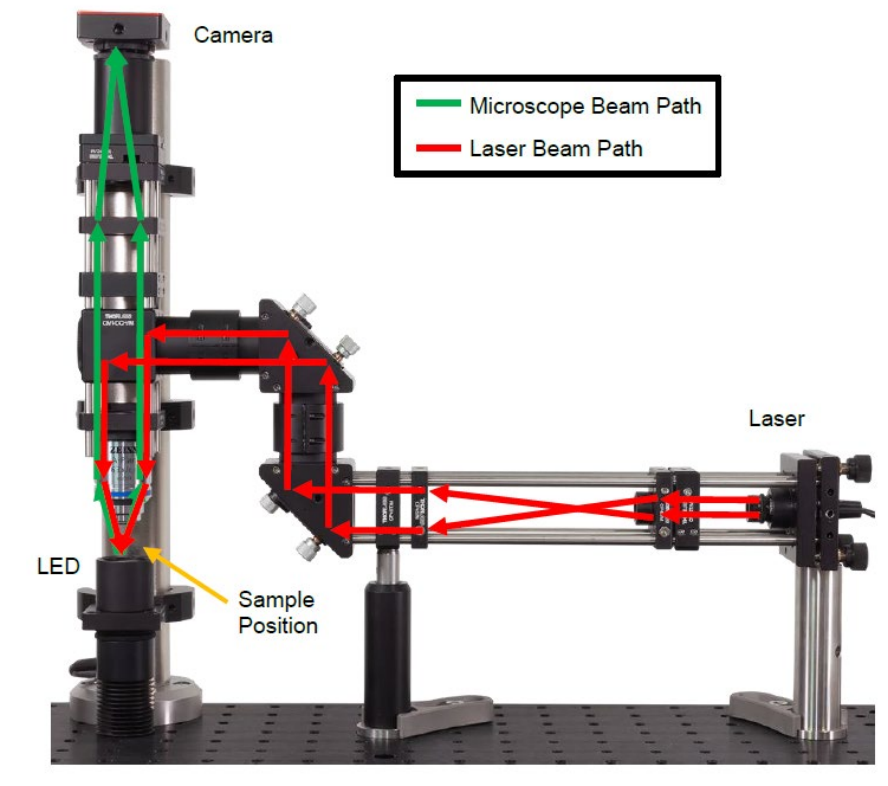
\includegraphics[width=\textwidth]{setup.png}
         \caption{Setup of the laser}
         \label{fig:setup}
     \end{subfigure}
     \hfill
     \begin{subfigure}[b]{0.45\textwidth}
         \centering
         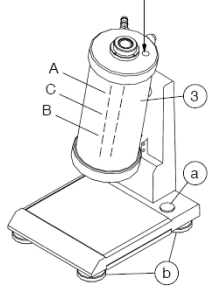
\includegraphics[width=0.65\textwidth]{viskosimeter.png}
         \caption{Falling sphere viscometer}
         \label{fig:three sin x}
     \end{subfigure}
     \hfill
        \caption{Experimental Setups}
        \label{fig:three graphs}
\end{figure}

As seen on figure \ref{fig:setup} the laser beam comes from the right side and travels trough several lenses, so that the focal plane of the laser and on the solution are nearly the same. Then it is introduced with a beam splitter and directed downwards to the sample. At the top of the setup is a camera to record the random movement of the particles in the solution, which is made visible with the microscope. The stage, where the sample is placed, can be moved around using the sample stage controllers. Additionally, the focus plane can be manipulated by changing the elevation of the objective. \\
The second experimental setup consists of a falling sphere viscometer, a reservoir filled with water. The viscosity of water can be determined by measuring the time a glass sphere takes to travel a certain distance inside the water.\\
Most part of this lab course will be conducted without the use of a laser.

\section{Method and Procedure}

\subsection{Calibration}
Before taking any measurements, the measurement software has to be calibrated. It is measuring the distance in pixels, and not in meters. The calibration is done by placing a small ruler with a grading of 10 $\mu$m beneath the optic of the microscope, and using the software's built-in tools, we establish the scale conversion from pixel to meter.

\subsection{Preparation of the silica samples}
In order to determine the Brownian movement of the silica particles, we first need to prepare the samples.\\
A double sided tape with a circular cutout in it's center is placed on a corner of a small glass piece. Then a drop of the silica solution is placed in the center of the circle using an Eppendorf pipette. To prevent evaporation, a thin glass plate is put on top of of the droplet. This procedure is done for 3 $\mu$m, 2$\mu$m and 6$\mu$m silica particles.

\subsection{Recording the Brownian movement of the particles}
Before starting the recording, the sample needs to be given 5-10 min in order to be seated properly. We make sure to focus the microscope on an area of the sample, where multiple particles can be clearly identified. Moreover the particles need to be isolated from other particles in its surroundings to avoid collisions, that would confuse the tracking software. When all the conditions are met, a recording of approximately 1 min is taken.\\
The video is exported to the software Tracker. We choose an appropriate particle, for which the movement is measured frame by frame, for the entire duration of the video. 

\subsection{Determination of the solution's viscosity by the study of the Brownian movement}
We export the data from the tracked particle to QTIplot. To calculate the displacement $\Delta x_i$, we have to set the column value to $x_{i+1} - x_i$ and covert it to $\mu$m by dividing this with the value found in the calibration part multiplied by the grading of the ruler (10 $\mu$m). The same can be done for $\Delta y_i$. Then we determine the horizontal displacement $r_i^2$ by setting the column value to $\Delta x_i^2 + \Delta y_i^2$.\\
The final step is to determine the average displacement $avg$ . To do so we have to set up the column value to $avg_{i-1}+r_i^2$. Now the average displacement can be plotted as a function of time. 

The movement is described by the Einstein-Smoluchowski equation:
\[\langle r^2\rangle=4D\cdot t\]
The slope of our graph, m, corresponds to 4D.
From the diffusion coefficient:
\[D=\frac{k_bT}{6\pi\eta_{eff}R}\]
an expression for the slope can be determined:
\begin{equation}
    m=\frac{2k_BT}{3\pi\eta_{eff}R}
    \label{equation_viscosity}
\end{equation}

From this equation, the viscosity of the solution $\eta_{eff}$ can be determined.

\subsection{Determination of the holding force}
The maximum holding force is given by:
\begin{equation}
    F_{max}=6\pi\eta_{eff}Rv_{max}
    \label{equ:force}
\end{equation}
In order to determine $v_{max}$, we look at the displacements in one dimension $\Delta x_i$ per time interval $t_{i+1}-t_{i}$, $\Delta t$. Then, using QtiPlot column statistics, the maximum value of $v_i$ is deduced. For the effective viscosity $n_{eff}$, we consider the average effective viscosity for each sample size found previously. For the magnitude of the holding force, a value of a few pN is expected.

\subsection{Determination of water's viscosity using a Falling sphere viscometer}
A glass bead is placed inside the apparatus filled with water. Then it is turned around and the time is measured from which the bead travels a certain distance marked by white lines. This is repeated a total of 5 times.
The viscosity can then be calculated using the following equation:
\begin{equation}
    \eta = k(\rho_{glass} -\rho_{water})\cdot t
    \label{equ_viscosity}
\end{equation}
With k = 0.00762, the density of glass $\rho_{glass}=2.5 \cdot 10^3 \ kg/m^3$  and the density of water $\rho_{water}=997 \ kg/m^3$. \\
Then we take the average time, in order to determine $\eta_{water}$.

\subsection{Trapping of a particle with the laser}
This part doesn't include any computation, since it is mostly there to discover how the optical tweezer work, by trapping particle with the laser. For this we use the sample containing the 3 $\mu$m silica particle and start the laser. The camera now shows a faded red dot, that is the laser, and by moving around the environment, we can capture a particle and moved it around as it is trapped by the laser light.

\section{Results}

\subsection{Determination of water's viscosity using a Falling sphere viscometer}
The recorded time are the following:
\[
\begin{array}{cc}
     t_1 = 1.51'28\\
     t_2 = 1.46'41\\
     t_3 = 1.45'79\\
     t_4 = 1.45'06\\
     t_5 = 1.44'98
\end{array}\]
The average time is therefore $\overline{t} = 104.2$ s.\\
The viscosity of water, using eq.~\ref{equ_viscosity} is $\boxed{\eta_{water} = 1.1934 \ \text{mPa $\cdot$ s}}$. 

The literature value of the viscosity is $\eta_{water,th}=1.0016 \ \text{mPa $\cdot$ s}$, so the value we determined has a 20\% deviation from the true viscosity of water.

\subsection{Determination of the prepared solutions' viscosity}
Here are some photographs of the particles taken by the camera:
\begin{figure}[H]
    \centering
    \begin{subfigure}{0.32\textwidth}
        \resizebox{\textwidth}{!}{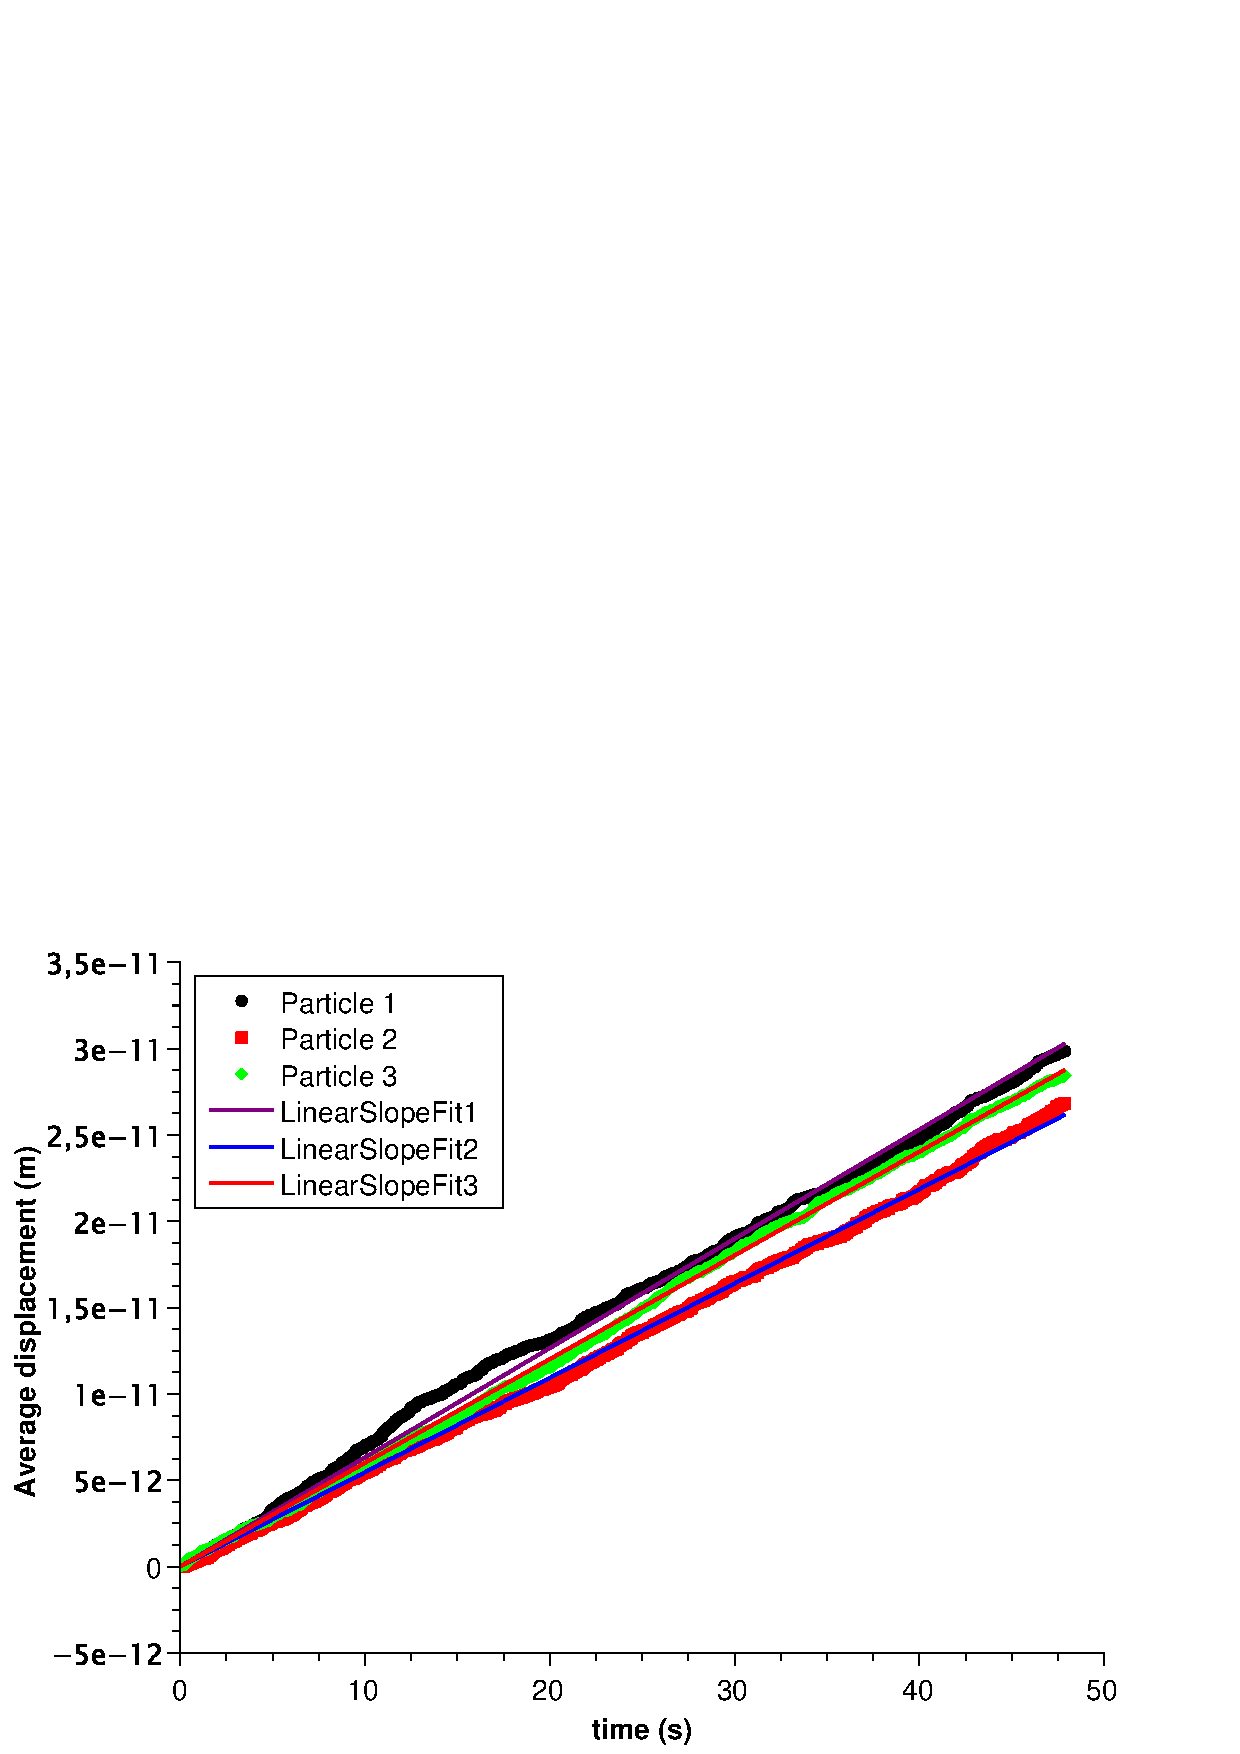
\includegraphics{2microns.png}}
        \caption{2 micron particles}
        \label{2micronsnap}
    \end{subfigure}
    \begin{subfigure}{0.32\textwidth}
        \resizebox{\textwidth}{!}{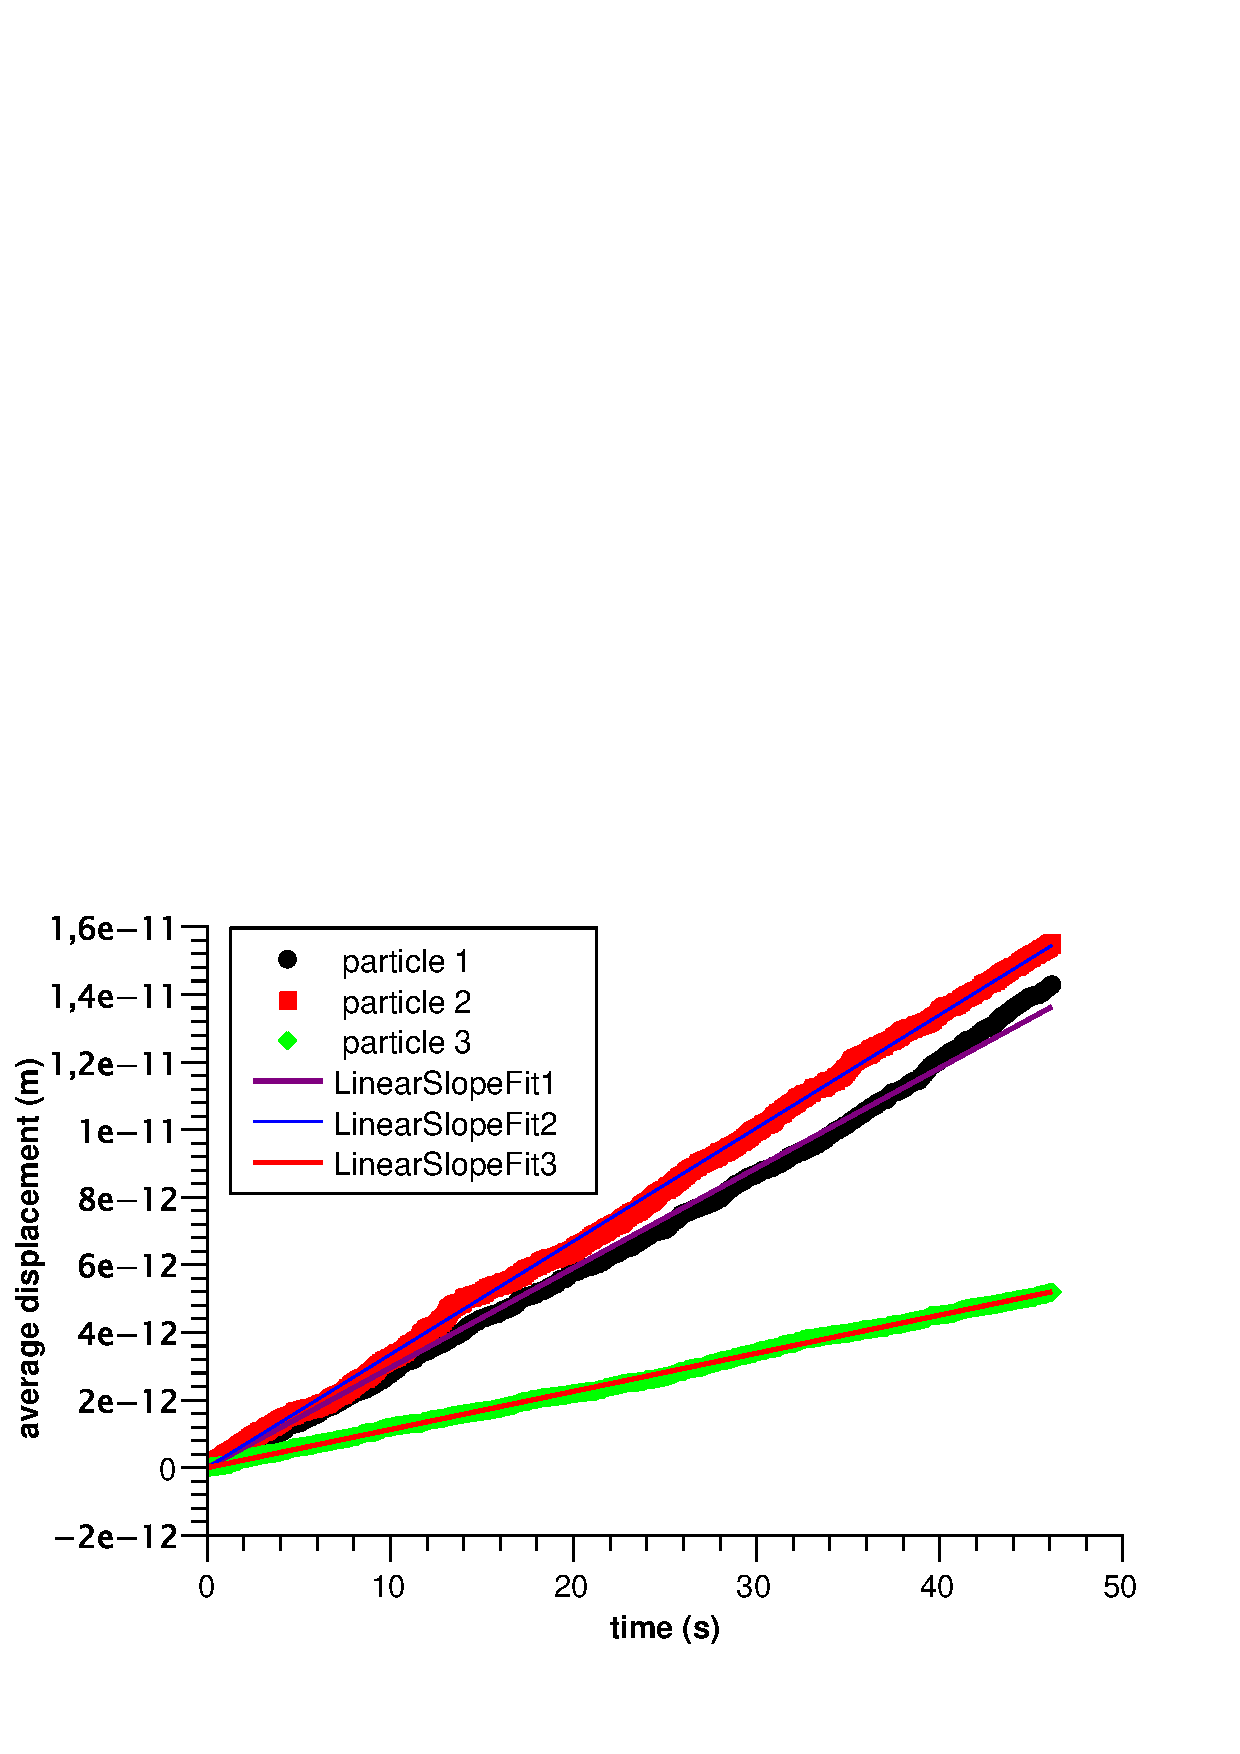
\includegraphics{3microns.png}}
        \caption{3 micron particles}
        \label{3micronsnap}
    \end{subfigure}
    \begin{subfigure}{0.32\textwidth}
        \resizebox{\textwidth}{!}{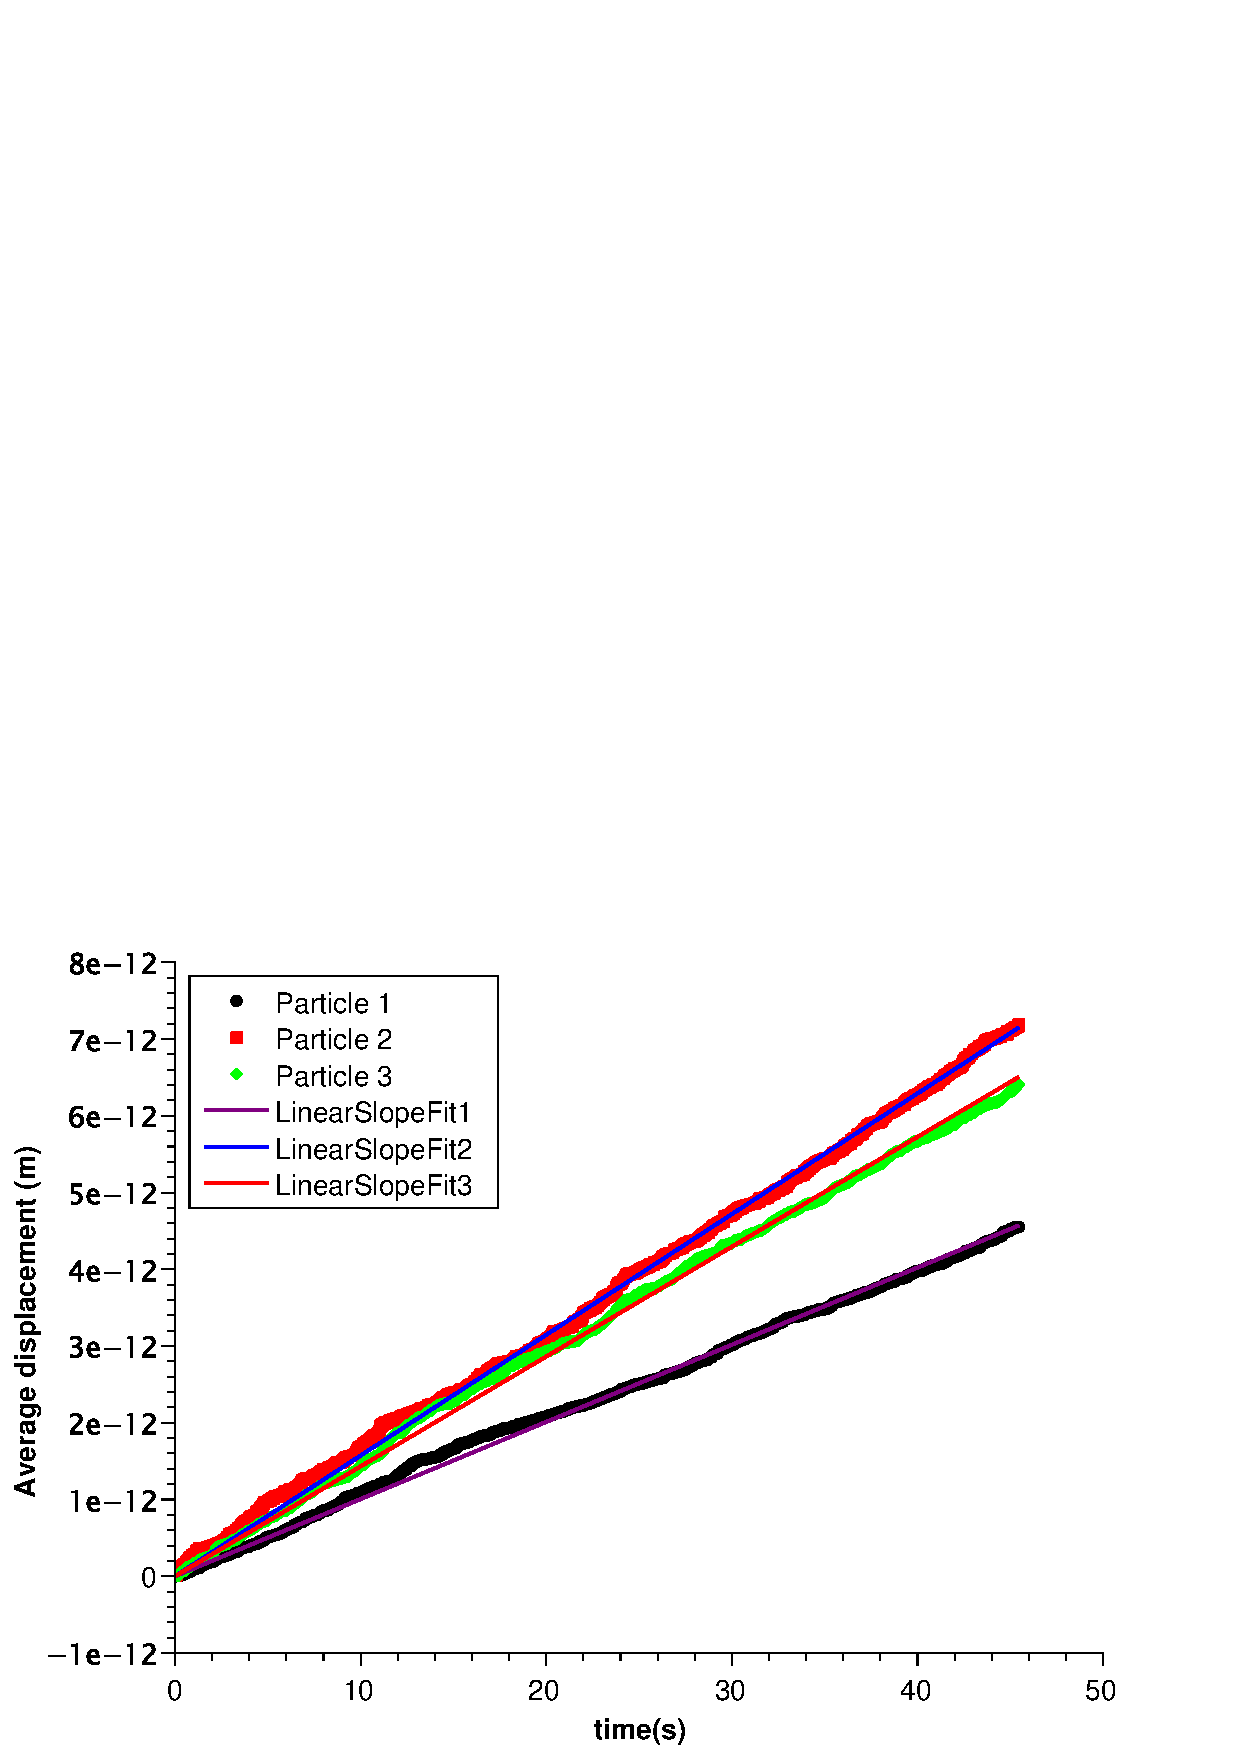
\includegraphics{6microns.png}}
        \caption{6 micron particles}
        \label{6micronsnap}
    \end{subfigure}
    \caption{Snapshots of the particles}
    \label{fig:snapshots}
\end{figure}

For later consideration, it is important to see at this point, that the solutions all seem to have different concentrations of beads, in terms of number of particles per volume. The photographs were all taken with the same optical zoom level. Oftentimes, there would be clusters of particles "glued" together, and for the study of the viscosity, only the motion individual beads, sufficiently separated from others so as not to be influenced by its neighbours, has to be tracked. While negligible, there is still some degree of freedom in the vertical movement of the beads. The Brownian motion is mostly happening in the horizontal plane however. \medskip

Using the procedure from section 4.4, we can determine the average displacement of each particle as a function of time.
\begin{figure}[H]
    \centering
    \includegraphics[width=0.8\textwidth]{qti/EVERYTHING.eps}
    \caption{Average displacement as a function of time for different particle sizes}
    \label{fig:my_label}
\end{figure}

As expected, we obtain linear relationships between the average displacement and time. The diagram shows that the general slope is different for each particle size. It decreases with increasing particle size. The reason for this is that larger particles move less in a medium.


\subsubsection{3 microns particles}
\begin{figure}[H]
    \centering
    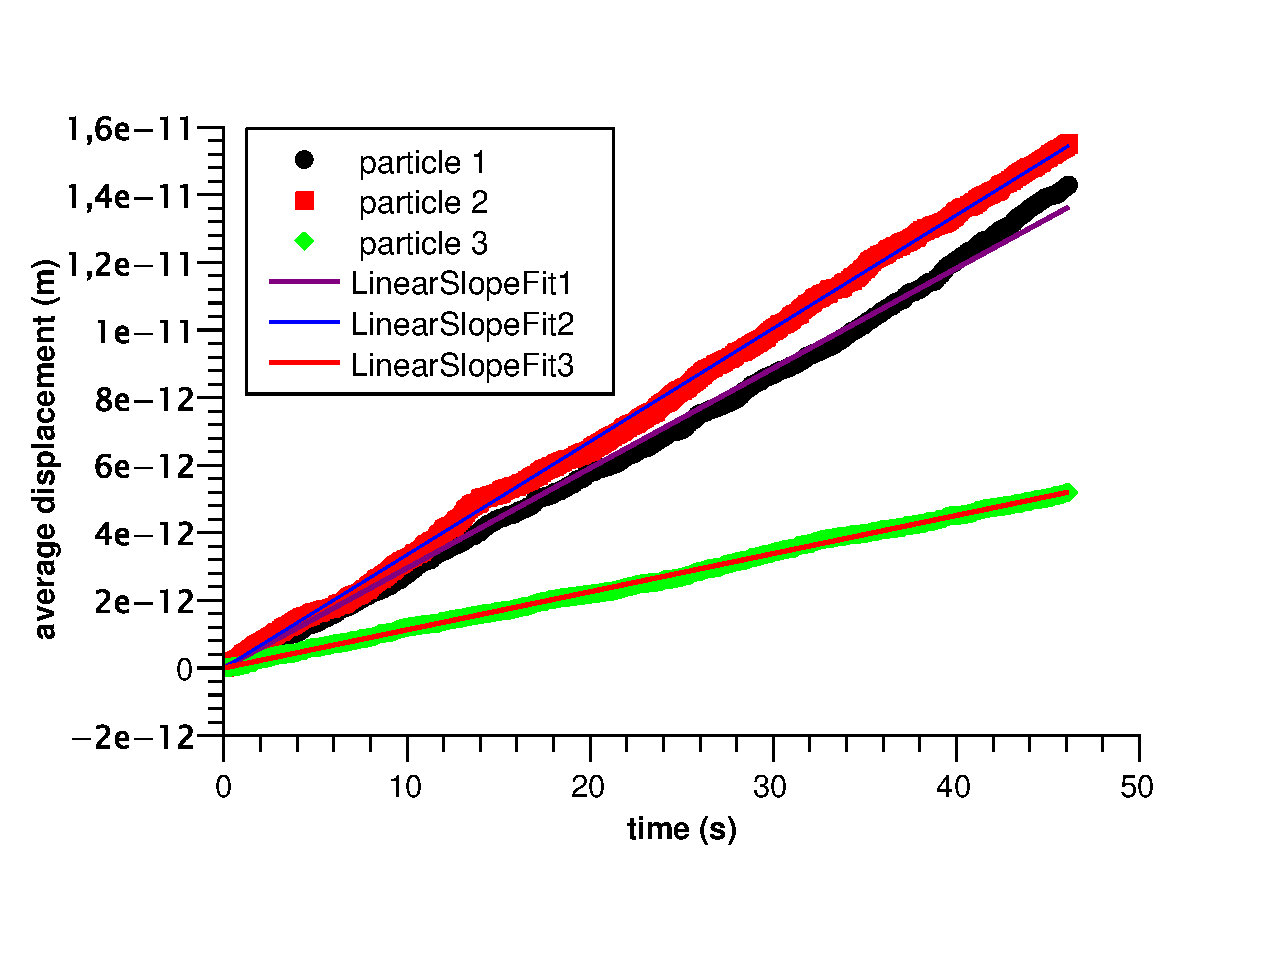
\includegraphics[width=0.7\textwidth]{qti/3microns.eps}
    \caption{average displacement as a function of time for 3 $\mu$m particles}
    \label{fig:3microns}
\end{figure}
As can be see, the third slope is not close enough to the others, meaning we can exclude this one from our calculation.\\
Using eq.~\ref{equ_viscosity}, we can express the viscosity of the solution, as:
\[ \eta_{eff} = \frac{2k_BT}{3\pi m R}\]
With T, the temperature, being 295,19 K (22°C), $k_B$ the Boltzmann constant and R the radius of the particle.\\

In the following table are listed the resulting slopes, as well as the calculated viscosity for each of them:
\begin{table}[H]
    \centering
    \begin{tabular}{c|c|c}
       Particle  & slope ($10^{-13}$ m$^2 \ \cdot$ s$^{-1}$ ) & Viscosity $\eta_{eff}$ (mPa $\cdot$ s) \\
       \hline
        1 & 2.95 & 1.95\\
        2 & 3.35 & 1.72
    \end{tabular}
    \caption{Resulting slope and calculated viscosity for each 3 $\mu$m particle }
    \label{tab:viscosity3micron}
\end{table}

The average viscosity is therefore: $\boxed{\overline{\eta}_{3\mu m} = 1.835 \ \text{mPa $\cdot$ s}}$ 

%The theoretical viscosity is more around 1 mPa $\cdot$ s at 20°C. Our tracking device is not precise enough, nevertheless, the experimental viscosity has the same order of magnitude.

\subsubsection{6 microns particles}
\begin{figure}[H]
    \centering
    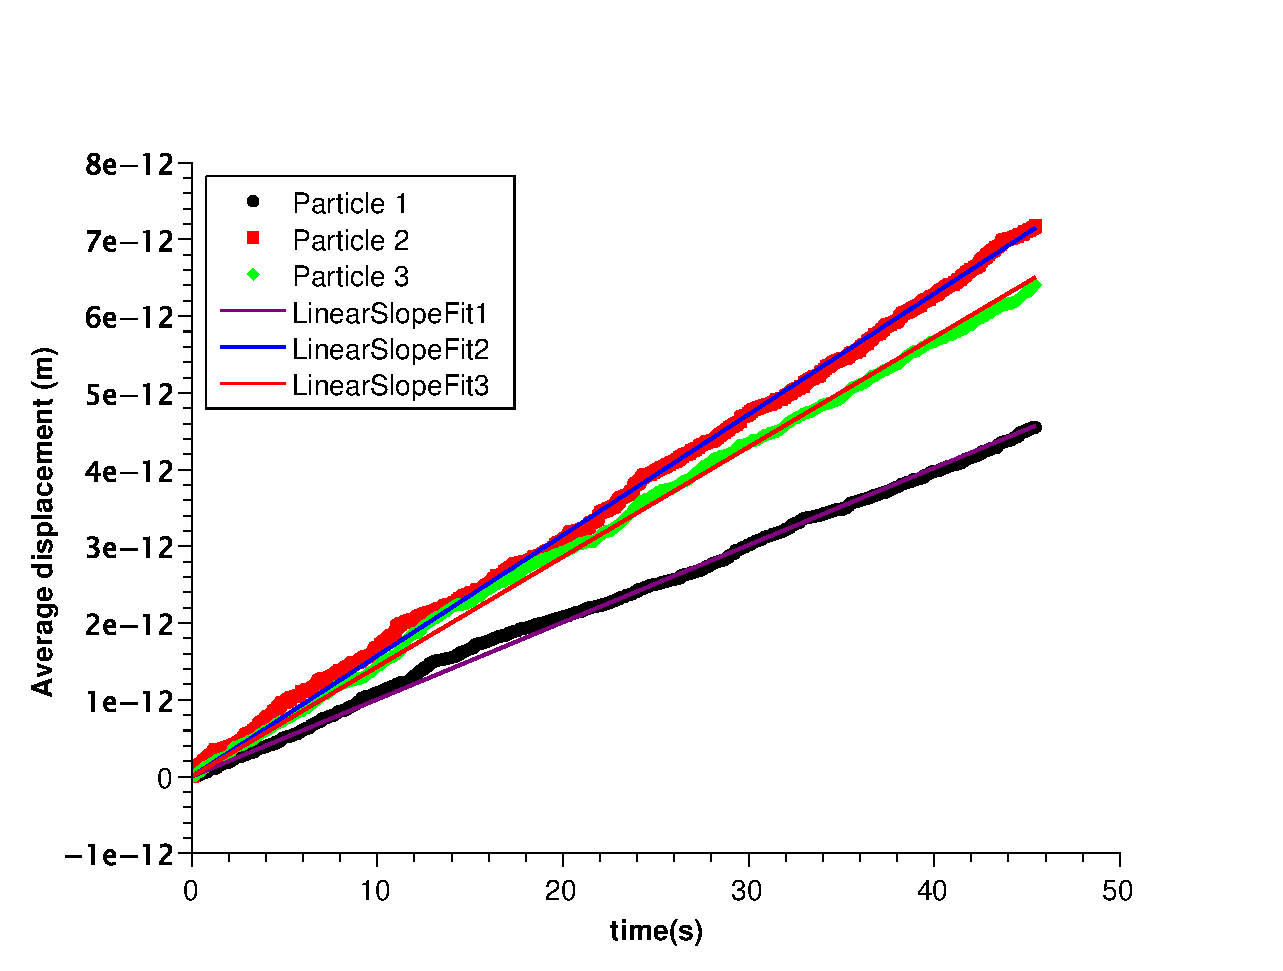
\includegraphics[width=0.7\textwidth]{qti/6microns.eps}
    \caption{average displacement as a function of time for 6 $\mu$m particles}
    \label{fig:6microns}
\end{figure}

\begin{table}[H]
    \centering
    \begin{tabular}{c|c|c}
       Particle  & slope ($10^{-13}$ m$^2 \cdot$ s$^{-1}$ ) & Viscosity $\eta_{eff}$ (mPa $\cdot$ s) \\
       \hline
        1 & 1.00 & 5.74\\
        2 & 1.57 & 3.68 \\
        3 & 1.43 & 4.03
    \end{tabular}
    \caption{Resulting slope and calculated viscosity for each 6 $\mu$m particle }
    \label{tab:viscosity6micron}
\end{table}

The average viscosity is therefore $\boxed{\overline{\eta}_{6\mu m} = 4.477 \ \text{mPa $\cdot$ s}}$ 

\subsubsection{2 microns particles}
\begin{figure}[H]
    \centering
    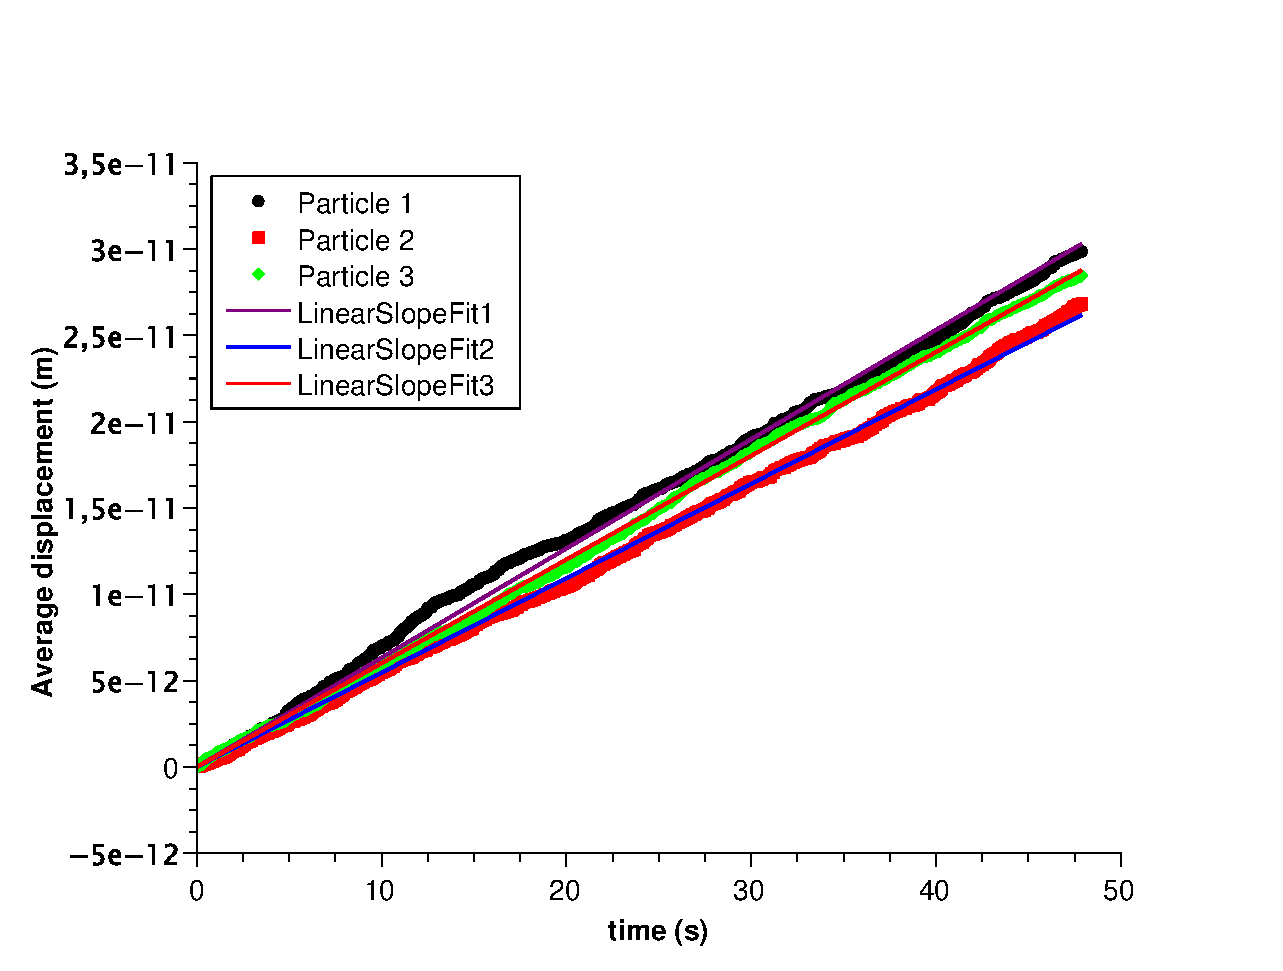
\includegraphics[width=0.7\textwidth]{qti/2microns.eps}
    \caption{average displacement as a function of time for 2 $\mu$m particles}
    \label{fig:2microns}
\end{figure}

\begin{table}[H]
    \centering
    \begin{tabular}{c|c|c}
       Particle  & slope ($10^{-13}$ m$^2 \cdot$ s$^{-1}$ ) & Viscosity $\eta_{eff}$ (mPa $\cdot$ s) \\
       \hline
        1 & 6.33 & 0.911\\
        2 & 5.47 & 1.05 \\
        3 & 6.01 & 0.959
    \end{tabular}
    \caption{Resulting slope and calculated viscosity for each 2 $\mu$m particle }
    \label{tab:viscosity2micron}
\end{table}
The average viscosity is therefore $\boxed{\overline{\eta}_{2\mu m} = 1.01 \ \text{mPa $\cdot$ s}}$ \medskip

When comparing the viscosities of the solutions with beads to the viscosity of water we previously determined, we notice that they are of the same order of magnitude, but that the beads have an influence on the viscosity. In general, the bigger the beads, the bigger the viscosity. This would need further study though, as the concentrations of beads in the solutions were not the same for the three particle sizes, as seen in fig.~\ref{fig:snapshots}.The viscosity then could also be, and certainly is, linked to the concentration of the beads in the solution.\vspace{0.5cm}

Now the holding force of the laser can be determined using equation \ref{equ:force}.
In the following table are listed the maximal velocities of each particle and for each particle size.
\begin{table}[H]
    \centering
    \begin{tabular}{c|c|c|c}
        Particle size & particle number & maximal velocity (m/s) & Holding force (N) \\
        \hline
        3 $\mu$m & 1 & 9.40 $\cdot 10^{-6}$ & 4.88$\cdot 10^{-13}$\\
        & 2 & 1.00 $\cdot 10^{-5}$ & 5.20 $\cdot 10^{-13}$ \\
        & 3 & 6.71 $\cdot 10^{-6}$ & 3.48 $\cdot 10^{-13}$\\
        \hline
        6 $\mu$m & 1 & 5.84 $\cdot 10^{-5}$ & 1.48 $\cdot 10^{-11}$ \\
        & 2 & 8.46 $\cdot 10^{-6}$ & 2.14 $\cdot 10^{-12}$\\
        & 3 & 5.95 $\cdot 10^{-6}$ &1.51 $\cdot 10^{-12}$\\
        \hline
        2 $\mu$m & 1 & 1.54 $\cdot 10^{-5}$ & 2.92 $\cdot 10^{-13}$ \\
        & 2 & 1.32 $\cdot 10^{-5}$ & 2.52 $\cdot 10^{-13}$\\
        & 3 & 1.54 $\cdot 10^{-5}$ & 2.92 $\cdot 10^{-13}$\\
    \end{tabular}
    \caption{ $v_{max}$ and holding force for each particle }
    \label{tab:my_label}
\end{table}

The average holding force for each particle size can now be determined:
\begin{align*}
    \overline{F}_{3\mu m} = 4.52 \cdot 10^{-13} \ N \\
    \overline{F}_{6\mu m} = 6.15 \cdot 10^{-12} \ N  \\
    \overline{F}_{2\mu m} = 2.79 \cdot 10^{-13} \ N
\end{align*}

As expected, our results for the average holding force is in the range of a few pico Newton. We can also observe, that the maximum holding force is smaller for smaller particles, which makes sense since smaller objects usually require less energy to be moved around. 

\section{Conclusion}
Overall the results we obtained during the lab session are satisfying as they lie at least in the correct order of magnitude. We we're able to quantify the influence of Brownian motion on the differently sized particles and thereby determine the effective viscosity of the solution they are suspended in. We noticed that the bigger the particle, the greater the effective viscosity becomes. Nevertheless, our results for the viscosity stayed between 1 and 4.5 mPa.s, and thus are in the same range of magnitude as the theoretical value. Moreover, we observed the trapping of the particles inside the laser beam and determined the maximum holding force it exerts.
\begin{thebibliography}{}
    \bibitem{labGuide} \textit{Optical tweezers - practical information}, Advanced lab class guide, Jörg Baller
    \bibitem{expGuide} \textit{Portable Optical Tweezers Educational Kit}, Online documentation, ThorLabs, \url{https://www.thorlabs.com/newgrouppage9.cfm?objectgroup_id=6966}, last accessed 28/05/2022 
    \bibitem{wiki} \textit{Optical Tweezer}, Wikipedia, \url{https://en.wikipedia.org/wiki/Optical_tweezers}, last accessed 28/05/2022
\end{thebibliography}

\end{document}
